\documentclass{article}
\usepackage[utf8]{inputenc}
\usepackage{graphicx}
\usepackage[style=ieee]{biblatex} % Establecer el estilo de las referencias como IEEE
\usepackage{xcolor}
\usepackage{hyperref}
\usepackage{titletoc}
\usepackage{adjustbox}
\usepackage[spanish]{babel}

\hypersetup{
    colorlinks=true,
    linkcolor=blue, % Color del texto del enlace
    urlcolor=blue % Color del enlace
}

\usepackage{longtable} % Agrega el paquete longtable

\definecolor{mygreen}{RGB}{0,128,0}

\usepackage{array} % Para personalizar la tabla
\usepackage{booktabs} % Para líneas horizontales de mejor calidad
\usepackage{float}
\usepackage[section]{placeins}

% Definir márgenes
\usepackage[margin=1in]{geometry}

\usepackage{listings}
\lstset{
    language=Python,
    basicstyle=\ttfamily\small,
    commentstyle=\itshape\color{gray},
    numbers=left,
    numbersep=5pt,
    tabsize=4,
    literate= % Permite tildes y ñ en el código
        {á}{{\'a}}1 {é}{{\'e}}1 {í}{{\'i}}1 {ó}{{\'o}}1 {ú}{{\'u}}1
        {Á}{{\'A}}1 {É}{{\'E}}1 {Í}{{\'I}}1 {Ó}{{\'O}}1 {Ú}{{\'U}}1
        {ñ}{{\~n}}1 {Ñ}{{\~N}}1
}

\renewcommand{\contentsname}{\textcolor{mygreen}{Tabla de Contenidos}}

\begin{document}

\begin{titlepage}
    \centering
    % Logo de la Universidad
    
\includegraphics[width=0.48\textwidth]{diagrams/logo_universidad.png}
    \par\vspace{2cm}

    % Nombre de la Universidad y detalles del curso
    {\Large \textbf{Universidad Nacional de Colombia} \par}
    \vspace{0.5cm}
    {\large Ingeniería de Sistemas y Computación \par}
    {\large 2025969 Modelos estocásticos y simulación en computación y comunicaciones (01)\par}
    \vspace{3cm}

    % Detalles del laboratorio y actividad
    {\large \textbf{Tarea 31} \par}
    {\large Más sobre el dilema del prisionero\par}
    \vspace{3cm}

    % Lista de integrantes
    {\large \textbf{Integrantes:} \par}
    \vspace{0.5cm}
    \begin{tabular}{ll}
    Javier Andrés Tarazona Jiménez & jtarazonaj@unal.edu.co \\
    Yenifer Yulieth Mora Segura & ymoras@unal.edu.co \\
    Jefferson Duvan Ramirez Castañeda & jeramirezca@unal.edu.co \\
    \end{tabular}
    \par\vspace{3cm}

    % Fecha
    {\large Junio 26 de 2025 \par}
\end{titlepage}

\tableofcontents % Inserta la tabla de contenidos

\newpage % Salto de página para separar la tabla de contenidos del contenido del documento

% Contenido del artículo----------------------------------------------------------

%---------------------------------------------------------------------------------
% Intro --------------------------------------------------------------------------
%---------------------------------------------------------------------------------

\section{Introducción}\label{sec:intr}

El Dilema del Prisionero es un paradigma clásico de la teoría de juegos que ilustra 
la tensión permanente entre interés individual y beneficio colectivo. 
En entornos estocásticos y sistemas distribuidos, este modelo proporciona un marco riguroso 
para analizar cómo agentes con distintos perfiles de comportamiento deciden cooperar o traicionar 
ante la incertidumbre y la interacción repetida.

El objetivo de esta tarea es profundizar en el estudio del Dilema del Prisionero a través 
de la implementación y confrontación de tres estrategias: la benévola \texttt{ElChance}, la 
malévola \texttt{Convenceme} y la clásica \texttt{TitForTat}. Mediante simulaciones iteradas 
de 200 rondas, se compararán sus historiales de puntajes, tasas de cooperación y 
victorias relativas, con el fin de determinar cuál de ellas ofrece un mejor 
equilibrio entre generosidad, represalia y claridad algorítmica.

%---------------------------------------------------------------------------------
% Marco Teórico ------------------------------------------------------------------
%---------------------------------------------------------------------------------

\section{Marco Teórico}\label{sec:marc}


\subsection{La Teoría de Juegos}
La teoría de juegos es la disciplina matemática que estudia las decisiones estratégicas de 
agentes interdependientes. Cada agente busca maximizar su propio beneficio, pero sus resultados 
dependen de las acciones de los demás. Los conceptos fundamentales incluyen:

\begin{itemize}
  \item \textbf{Jugadores}: agentes que toman decisiones.
  \item \textbf{Estrategias}: conjunto de acciones posibles para cada jugador.
  \item \textbf{Pagos (Payoffs)}: recompensas o pérdidas asociadas a cada combinación de 
    estrategias.
  \item \textbf{Equilibrio de Nash}: situación en la que ningún jugador puede mejorar 
    su pago cambiando unilateralmente su propia estrategia.
  \item \textbf{Estrategia Dominante}: Para cada jugador, no cooperar (traicionar) es mejor 
    sin importar la decisión del otro.
\end{itemize}

\subsection{Definición del Dilema del Prisionero}
El Dilema del Prisionero es un juego no cooperativo de dos jugadores, con las siguientes
características:

\begin{enumerate}
  \item \textbf{Hipótesis básica}: dos individuos aislados no pueden comunicarse.
  \item \textbf{Opciones de estrategia}: cooperar (\emph{guardar silencio}) o 
    traicionar (\emph{confesar}) - no cooperar.
  \item \textbf{Matriz de pagos}:\newline
  \begin{itemize}
    \item Ambos cooperan: pena moderada para cada uno.
    \item Uno coopera, otro traiciona: el traidor sale libre, el cooperador recibe la pena máxima.
    \item Ambos traicionan: pena intermedia para cada uno.
  \end{itemize}
\end{enumerate}

Matemáticamente, si denotamos la recompensa por mutua cooperación como $R$, 
la tentación de traicionar como $T$, la sanción por traición mutua como $P$ y la poca recompensa 
por ser traicionado como $S$, se cumple la desigualdad:

\[
T > R > P > S.
\]

\subsection{Estrategias y Equilibrio}
\begin{itemize}
  \item \textbf{Estrategia dominante}: para cada jugador, "traicionar" maximiza el pago 
    independiente de la decisión del otro.
  \item \textbf{Equilibrio de Nash}: $(traicionar / traicionar)$, aunque el resultado 
    colectivo óptimo sería la cooperación mutua.
\end{itemize}

\subsection{Extensiones y Repetición de Juegos}
Para modelar dinámicas más realistas, se considera el juego repetido:

\begin{itemize}
  \item \textbf{Repetición finita}: descompone la cooperación escalonada.
  \item \textbf{Repetición indeterminada}: permite estrategias condicionadas 
    (por ejemplo, \emph{Tit for Tat}), que fomentan la cooperación sostenida.
\end{itemize}

\subsection{Aplicación en Modelos Estocásticos y Simulación}
En sistemas de comunicaciones, el Dilema del Prisionero se emplea para:

\begin{itemize}
  \item Analizar protocolos de cooperación entre nodos (por ejemplo, reenvío de paquetes).
  \item Evaluar mecanismos de castigo y reputación.
  \item Explorar políticas de enrutamiento colaborativo bajo incertidumbre.
\end{itemize}

La simulación estocástica permite cuantificar cómo varían las tasas de cooperación 
según parámetros de castigo, beneficio y horizonte temporal.

%---------------------------------------------------------------------------------
% Descripción y Justificación del Problema a Resolver ----------------------------
%---------------------------------------------------------------------------------

\section{Descripción y Justificación del Problema a Resolver}\label{sec:descr}

En esta tarea se profundiza en el Dilema del Prisionero desde una perspectiva complementaria a 
la presentada en clase. Para ello, con base al episodio titulado “Lo que el Dilema del 
Prisionero Revela Sobre la Vida, el Universo y Todo lo Demás”, del canal Veritasium, en el 
que el Dr. Muller ilustra con ejemplos prácticos cómo distintas estrategias interactúan en 
un juego iterado de cooperación versus traición [\ref{ref:vidIntro}].

En principio se debe:
\begin{itemize}
  \item Revisar y analizar el contenido audiovisual propuesto, comprendiendo los fundamentos 
    del Dilema del Prisionero y la dinámica de las estrategias exhibidas 
    (especialmente la estrategia “Tit for Tat”).

  \item Diseñar y codificar dos nuevas estrategias propias

  \item Una benévola, que tienda a favorecer la cooperación inicial y perdonar 
    ocasionalmente la traición del oponente.

  \item Una malévola, que aproveche al máximo las oportunidades para traicionar al adversario, 
    buscando maximizar su propio beneficio.

  \item Implementar un simulador estocástico, donde cada par de estrategias 
    (benévola vs. Tit for Tat, malévola vs. Tit for Tat, y benévola vs. malévola) 
      se enfrente en múltiples rondas sucesivas bajo el esquema clásico de penalizaciones y 
      recompensas del Dilema del Prisionero.

  \item Estimar la eficacia de cada estrategia midiendo, a través de estadísticas de simulación, 
    el promedio de "pago" obtenido (nivel de cooperación lograda o traiciones realizadas) 
      en condiciones repetidas.

  \item El desafío consiste en traducir esos principios teóricos y audiovisuales a un 
  experimento computacional para definir cual es el enfoque mas eficiente.
\end{itemize}


El Dilema del Prisionero no solo es un pilar de la teoría de juegos, sino que en la práctica 
constituye un modelo esencial para simular el comportamiento de agentes en entornos estocásticos. 
Sus aplicaciones abarcan desde redes de comunicación distribuidas y protocolos de reenvío de 
paquetes hasta procesos evolutivos, dinámicas humanas de conflicto y competición en múltiples 
ámbitos. Entenderlo a fondo y experimentar con estrategias diversas es clave para diseñar 
sistemas robustos y predecir comportamientos en escenarios complejos.

En concreto, El Dilema sirve como un paradigma clave en simulaciones multiagente para modelar 
decisiones de cooperación y conflicto en entornos estocásticos, donde agentes con 
comportamientos pavlovianos y estrategias diversas interactúan en redes espaciales complejas 
para reproducir dinámicas reales de comunicación y competencia .
En sistemas distribuidos, esta lógica inspira protocolos de reenvío de paquetes y mecanismos de 
reputación que refuerzan o castigan conductas según el historial de cooperación.
Por su parte, en biología evolutiva, el juego explica la emergencia de comportamientos altruistas 
y de enjambre bajo presión selectiva.
Del mismo modo, la teoría se extiende a dinámicas humanas y bélicas, como el “security dilemma”, 
donde medidas defensivas generan espirales de desconfianza estatal, como la guerra fría. Pero
en ámbitos competitivos como el deporte y la economía, retrata por qué las estrategias 
egoístas conducen a resultados colectivos subóptimos. Finalmente, 
la experimentación mediante simulaciones iteradas permite calibrar parámetros de castigo, 
beneficio y perdón desde enfoques benignos hasta agresivos para diseñar protocolos robustos 
en sistemas ad hoc y distribuidos, fusionando teoría de juegos con práctica 
computacional avanzada [\ref{ref:just}].

%---------------------------------------------------------------------------------
% Diseño de la solución ---------------------------------------------------------
%---------------------------------------------------------------------------------

\section{Diseño de la solución}\label{sec:dis}

% Diseño de Solución para el simulador de agentes en el Dilema del Prisionero
\section*{Diseño de Solución}

El sistema se organiza en torno a una jerarquía de clases que modelan agentes capaces de jugar iteraciones del 
Dilema del Prisionero, junto con un módulo de simulación ("torneo") que empareja y hace competir a estos agentes. 
La solución consta de los siguientes componentes:

\begin{enumerate}
  \item \textbf{Estructura de Clases:} Ver imagen \ref{fig:class_diag}.
    \begin{description}
      \item[Clase base \texttt{Agente}] Define el comportamiento común a todos los jugadores:
        \begin{itemize}
          \item \emph{Atributos:}
            \begin{itemize}
              \item \texttt{state (int)}: última acción tomada (COOP o NOT\_COOP).
              \item \texttt{rounds\_played (int)}: número de rondas ya jugadas.
              \item \texttt{prev\_opponent\_response (Optional[int])}: respuesta anterior del oponente.
              \item \texttt{opponent\_consec\_count (int)}: conteo de respuestas idénticas consecutivas del oponente.
            \end{itemize}
          \item \emph{Métodos:}
            \begin{itemize}
              \item \texttt{start() -> int}: inicializa los contadores y devuelve la acción de la primera ronda.
              \item \texttt{choose(prev\_opponent\_response: int) -> int}: actualiza el estado interno, valida la respuesta del rival y elige la siguiente acción.
              \item \texttt{\_validate\_response(...)}: comprueba que la señal recibida sea COOP o NOT\_COOP.
              \item \texttt{\_choose\_coop()} y \texttt{\_choose\_not\_coop()}: manejan la lógica de cambio de \texttt{state} cuando el agente está en modo cooperar o no cooperar.
            \end{itemize}
        \end{itemize}
      \item[Subclases concretas]
        \begin{description}
          \item[\texttt{ElChance} (benévola):]
            \begin{itemize}
              \item Primera ronda: coopera siempre.
              \item Cuando coopera: sigue cooperando con probabilidad 95\%, 5\% de aleatoriedad. Si el oponente no coopera dos rondas seguidas, cambia a NO\_COOP.
              \item Cuando no coopera: permanece en NO\_COOP hasta que el oponente coopere, pero con probabilidad 10\% decide perdonar y cooperar.
            \end{itemize}
          \item[\texttt{Convenceme} (malévola):]
            \begin{itemize}
              \item Primera ronda: NO\_COOP.
              \item Cuando no coopera: mantiene NO\_COOP hasta que el oponente coopere, salvo una probabilidad 5\% de "piedad" donde coopera.
              \item Cuando coopera: lo hace al menos dos rondas, si el oponente vuelve a traicionar, regresa a NO\_COOP, tras cualquier par de cooperaciones, puede castigar con 10 rondas de NO\_COOP.
            \end{itemize}
          \item[\texttt{TitForTat}:]
            \begin{itemize}
              \item Primera ronda: COOP.
              \item Si el oponente cooperó, coopera, si traicionó, traiciona.
            \end{itemize}
        \end{description}
    \end{description}

  \item \textbf{Módulo de Simulación ("Torneo")}\\
    \texttt{torneo(agentes: List[Agente], n\_rondas: int) -> Resultados}
    \begin{enumerate}
      \item \emph{Inicialización:} para cada agente se invoca \texttt{start()} y se almacena la acción inicial.
      \item \emph{Iteración de rondas (2 a n\_rondas):}
        \begin{itemize}
          \item Para cada par ordenado $(A,B)$:
            \begin{enumerate}
              \item $a = A.choose(prev\_B)$ usando la última respuesta de $B$.
              \item $b = B.choose(prev\_A)$ usando la última respuesta de $A$.
              \item Registrar pagos según la matriz y actualizar historiales.
            \end{enumerate}
        \end{itemize}
      \item \emph{Cálculo de métricas:} al finalizar, para cada agente:
        \begin{itemize}
          \item Puntuación total (suma de pagos).
          \item Tasa de cooperación (n\_COOP / n\_rondas).
          \item Victorias relativas (veces con mayor pago).
        \end{itemize}
    \end{enumerate}

  \item \textbf{Flujo de Ejecución}
    \begin{enumerate}
      \item Definir instancias de \texttt{ElChance}, \texttt{Convenceme} y \texttt{TitForTat}.
      \item Configurar torneo: número de rondas y tipo de emparejamientos.
      \item Ejecutar \texttt{torneo(...)} y recolectar resultados.
      \item Analizar resultados (tablas o gráficos con \texttt{matplotlib} o \texttt{pandas}).
    \end{enumerate}

\end{enumerate}

\begin{figure}[H]        
  \centering             
  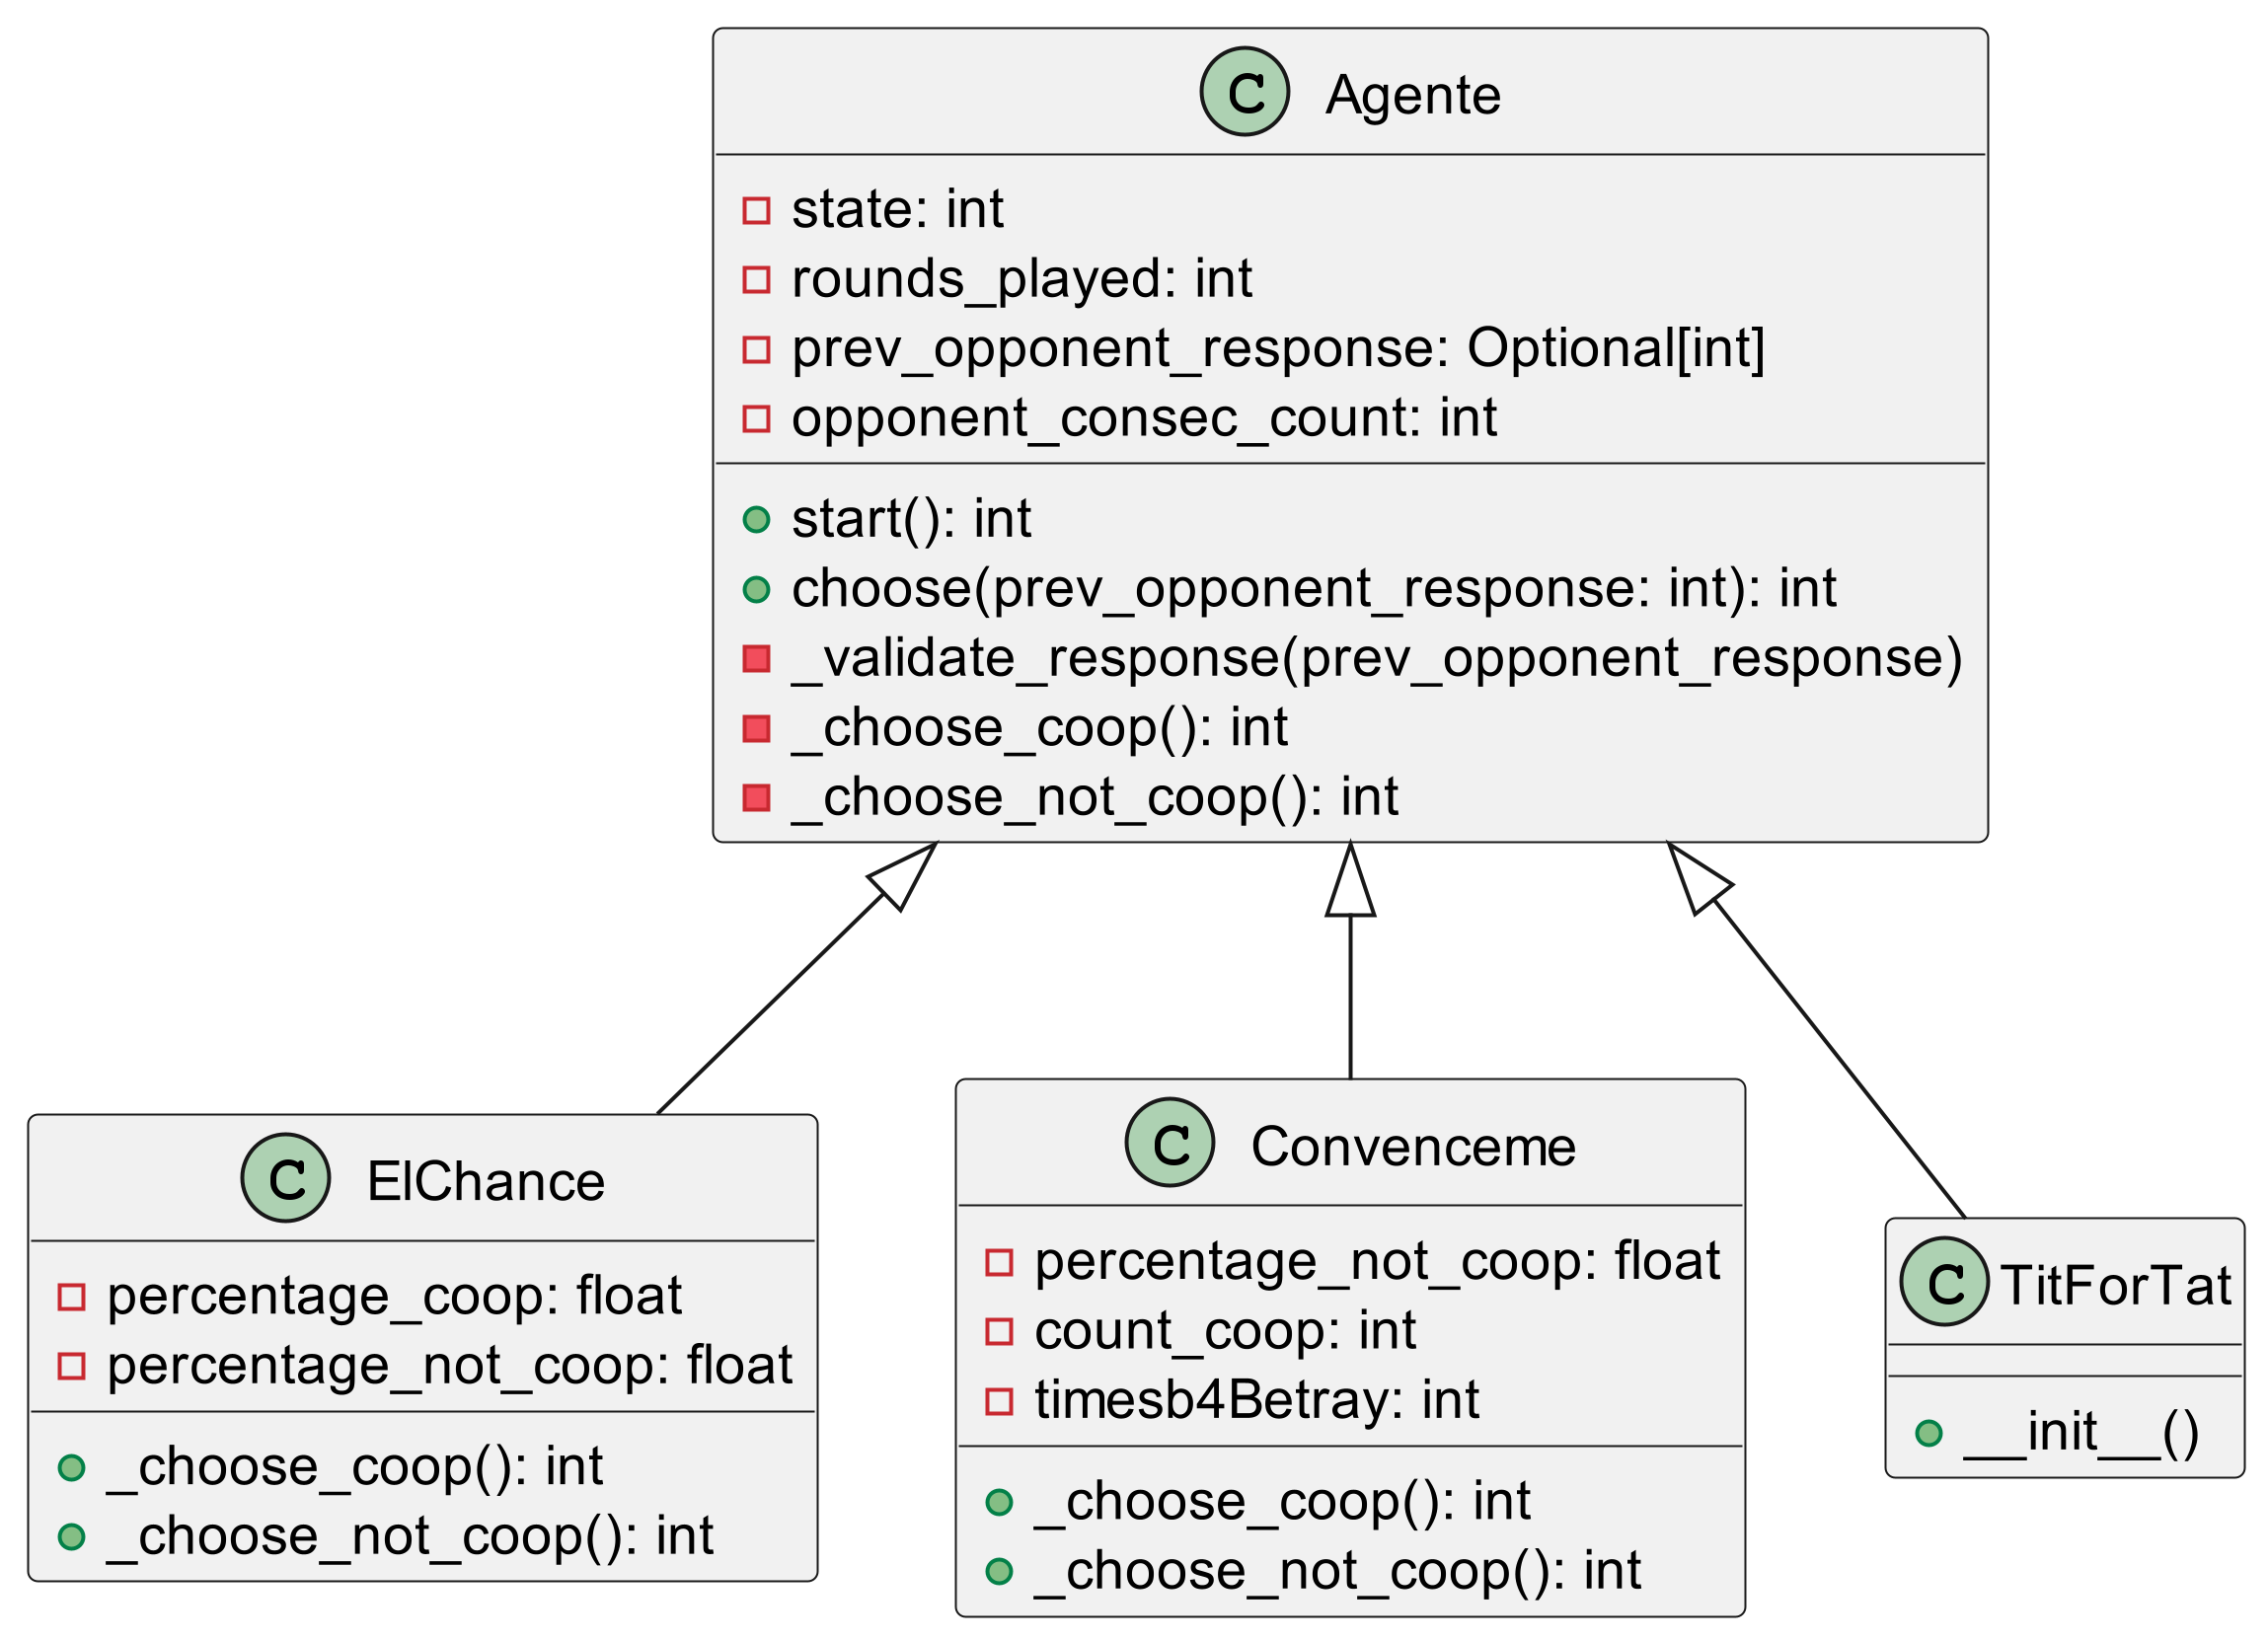
\includegraphics[width=0.96\textwidth]{diagrams/class_diag.png}
  \caption{Diagrama de clases}
  \label{fig:class_diag}
\end{figure}

\begin{figure}[H]        
  \centering             
  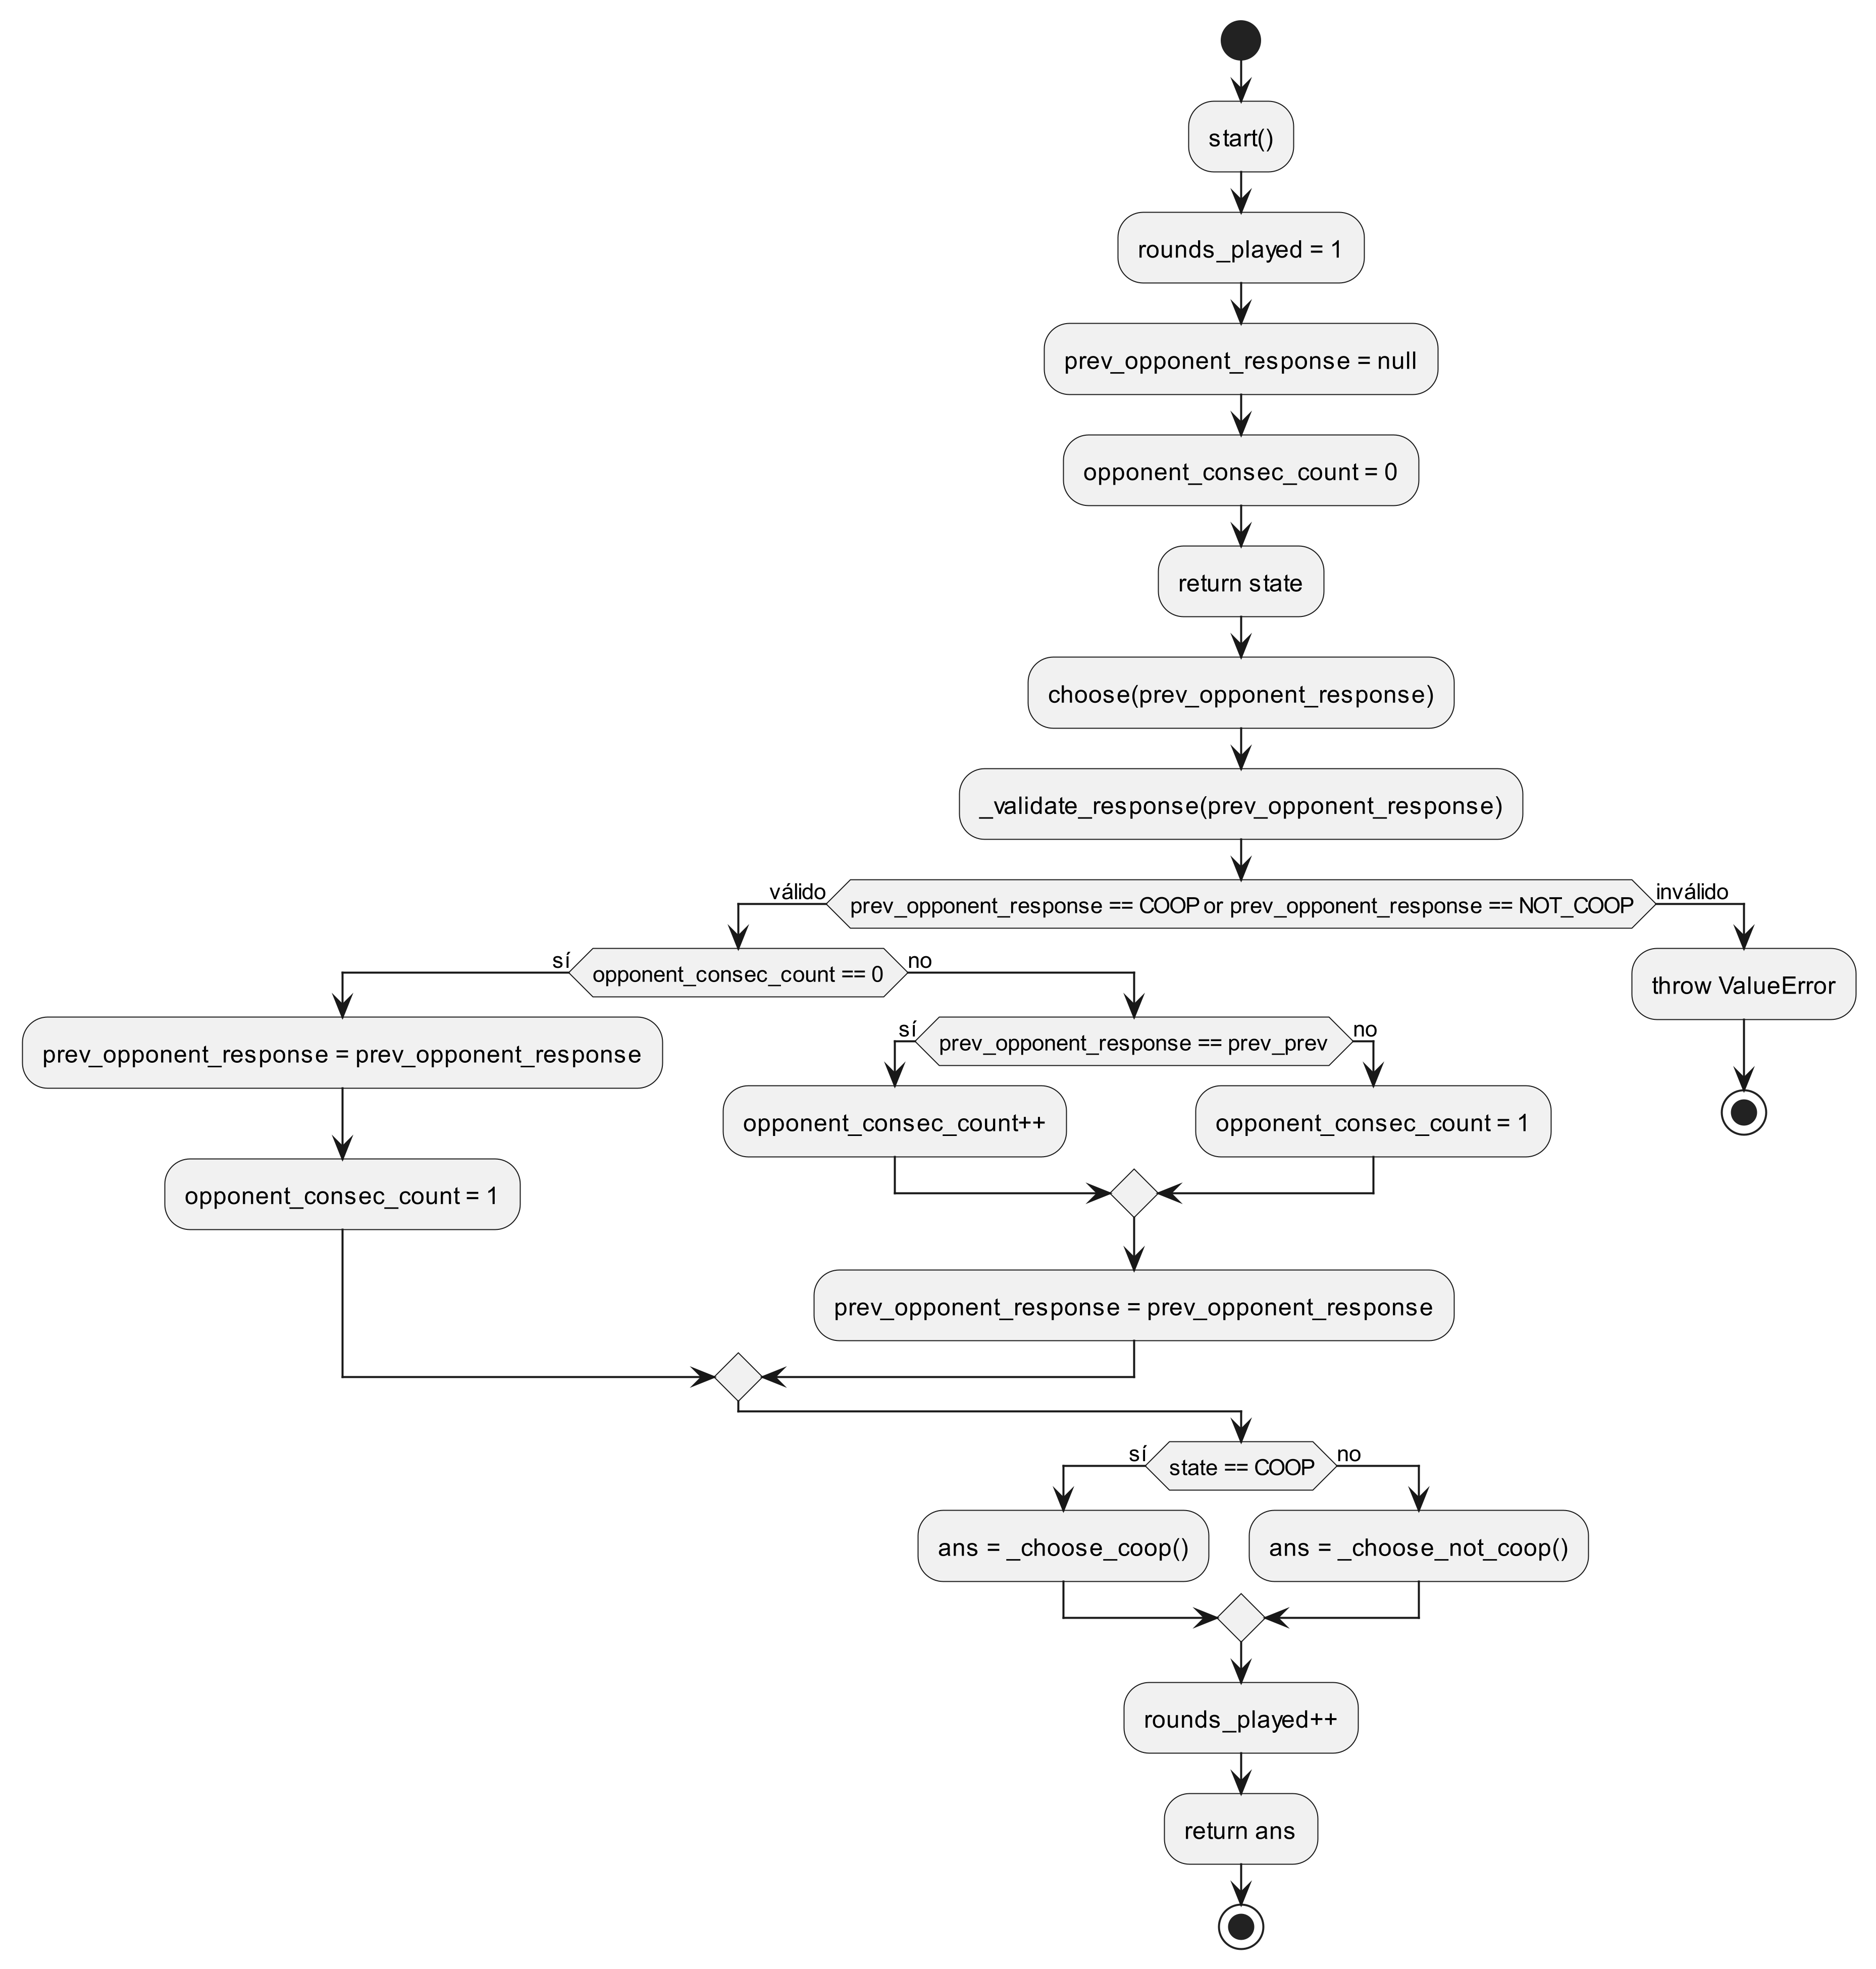
\includegraphics[width=0.96\textwidth]{diagrams/flow_diag.png}
  \caption{Diagrama de actividad del flujo de los agentes}
  \label{fig:flow_diag}
\end{figure}

\begin{figure}[H]        
  \centering             
  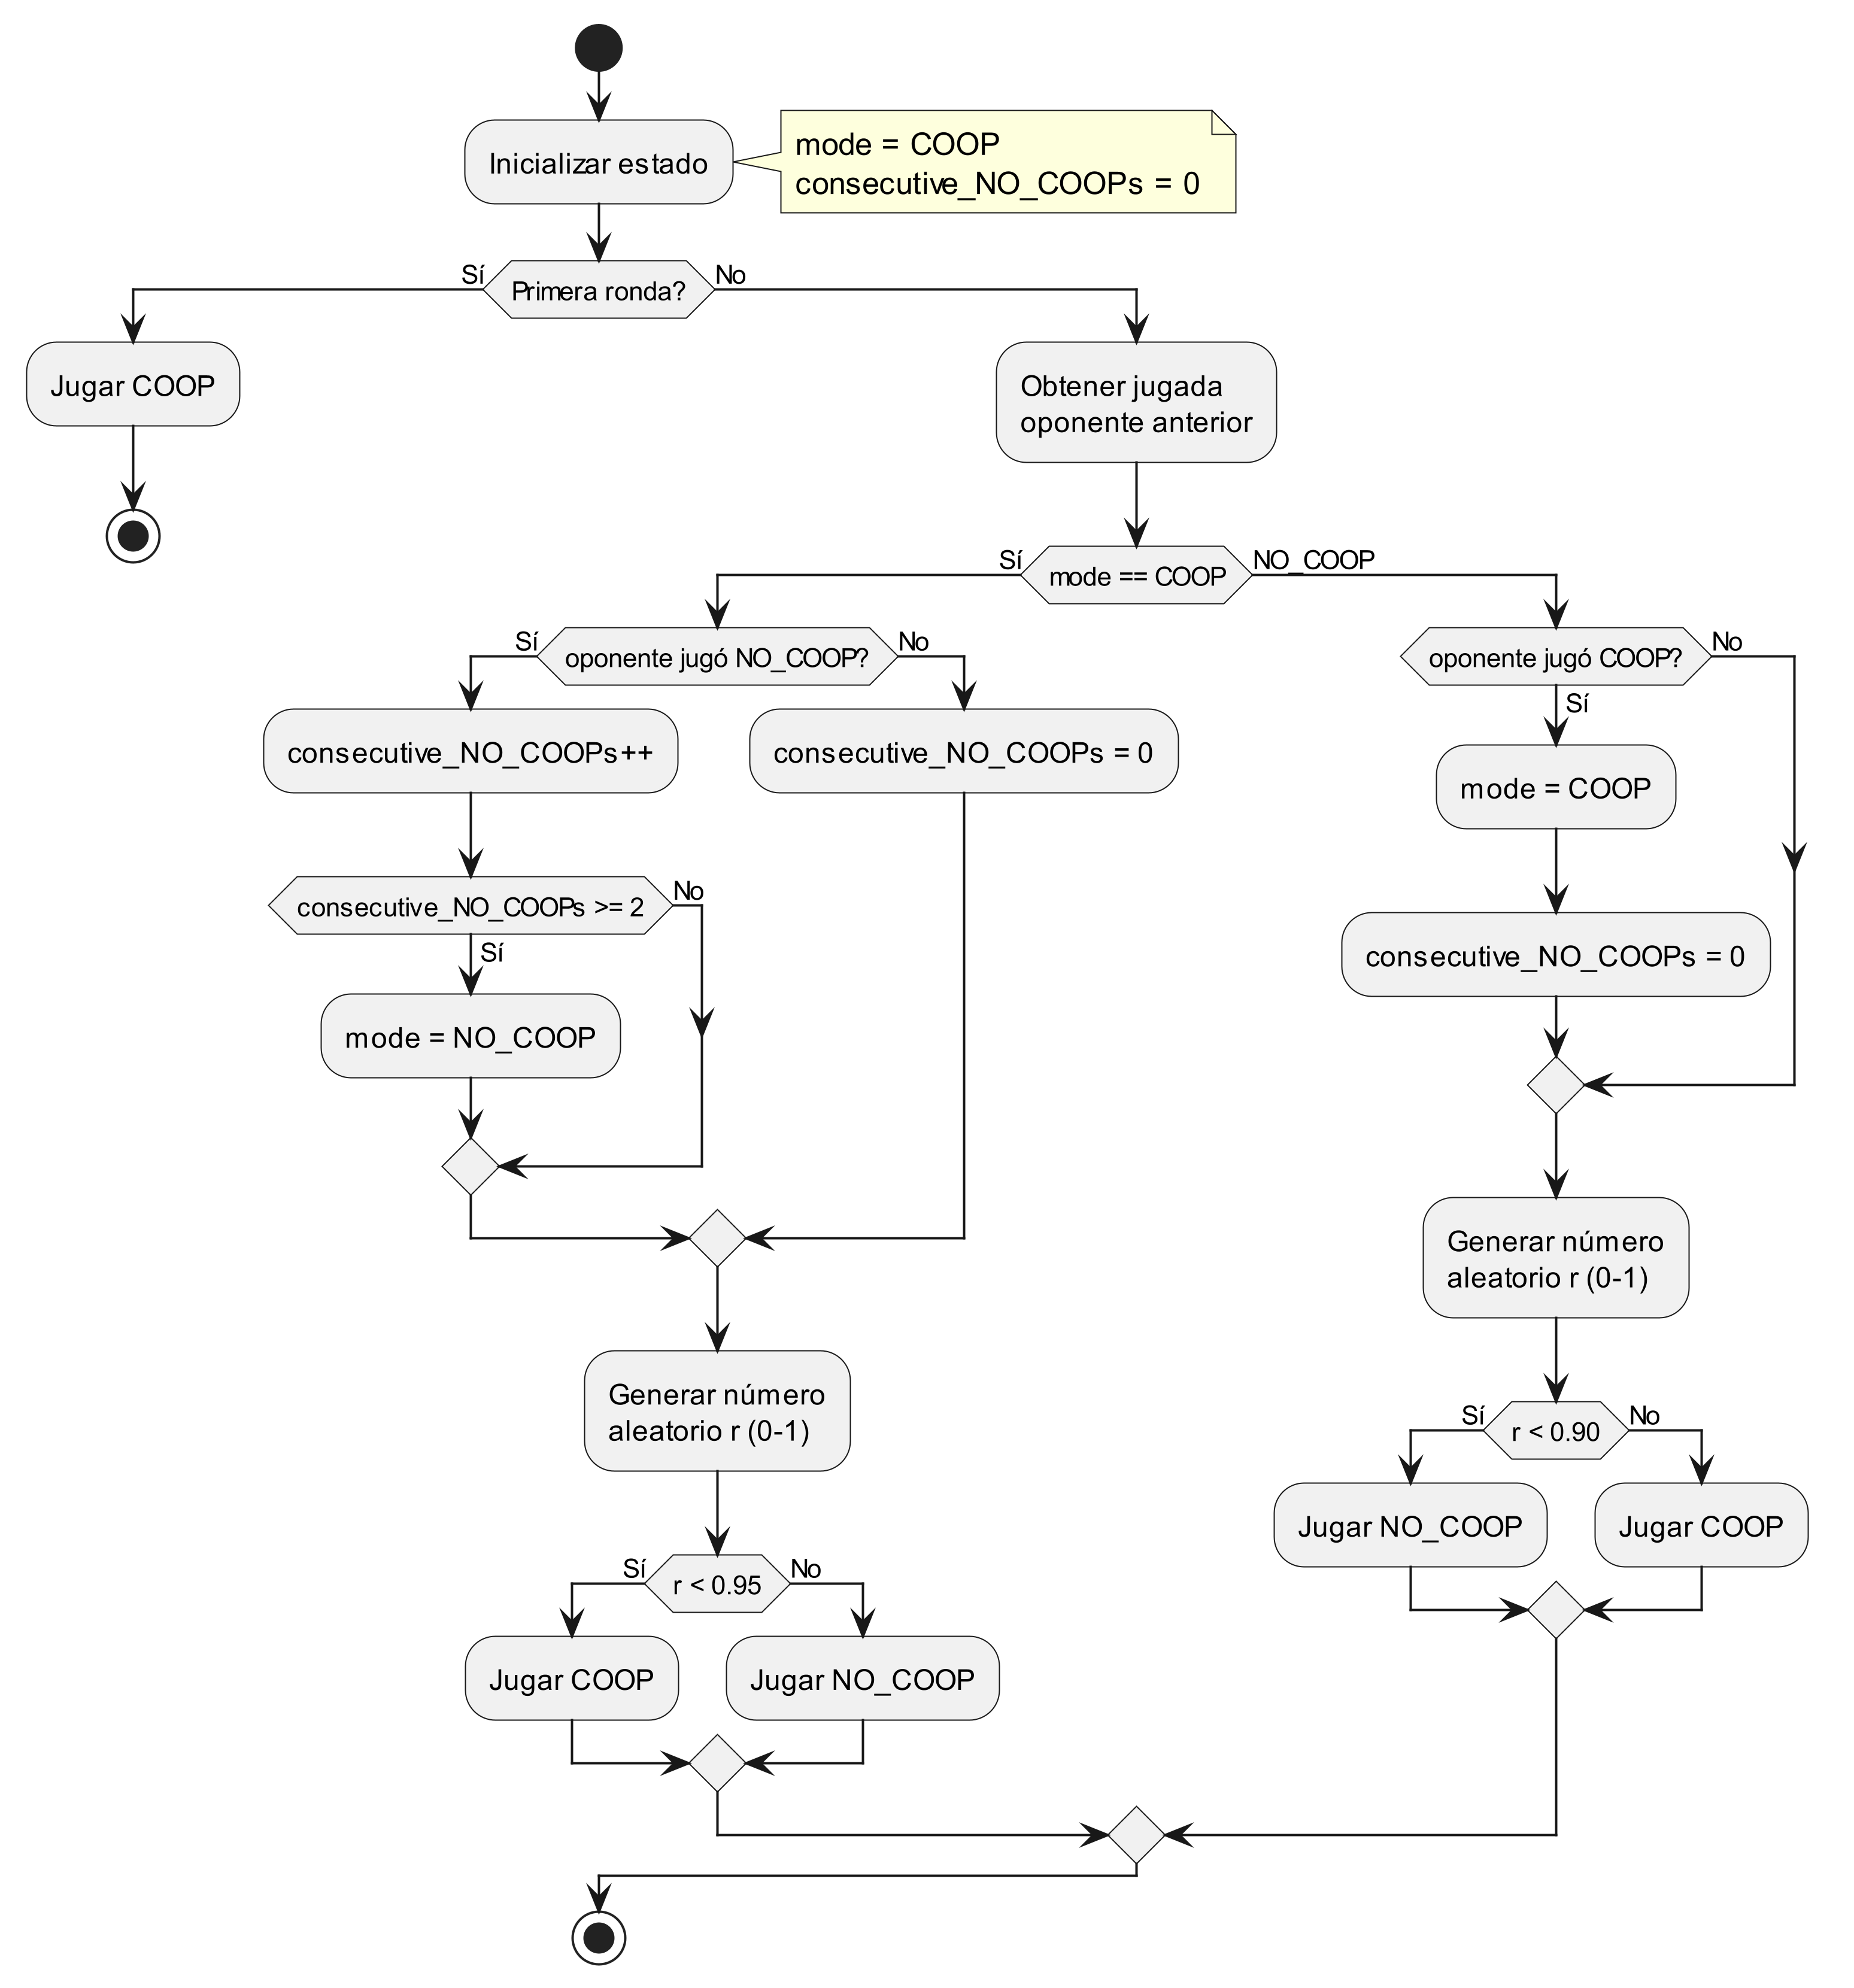
\includegraphics[width=0.96\textwidth]{diagrams/flow_chance.png}
  \caption{Diagrama de actividad del flujo del agente agente benévolo: ElChance}
  \label{fig:low_chance}
\end{figure}

\begin{figure}[H]        
  \centering             
  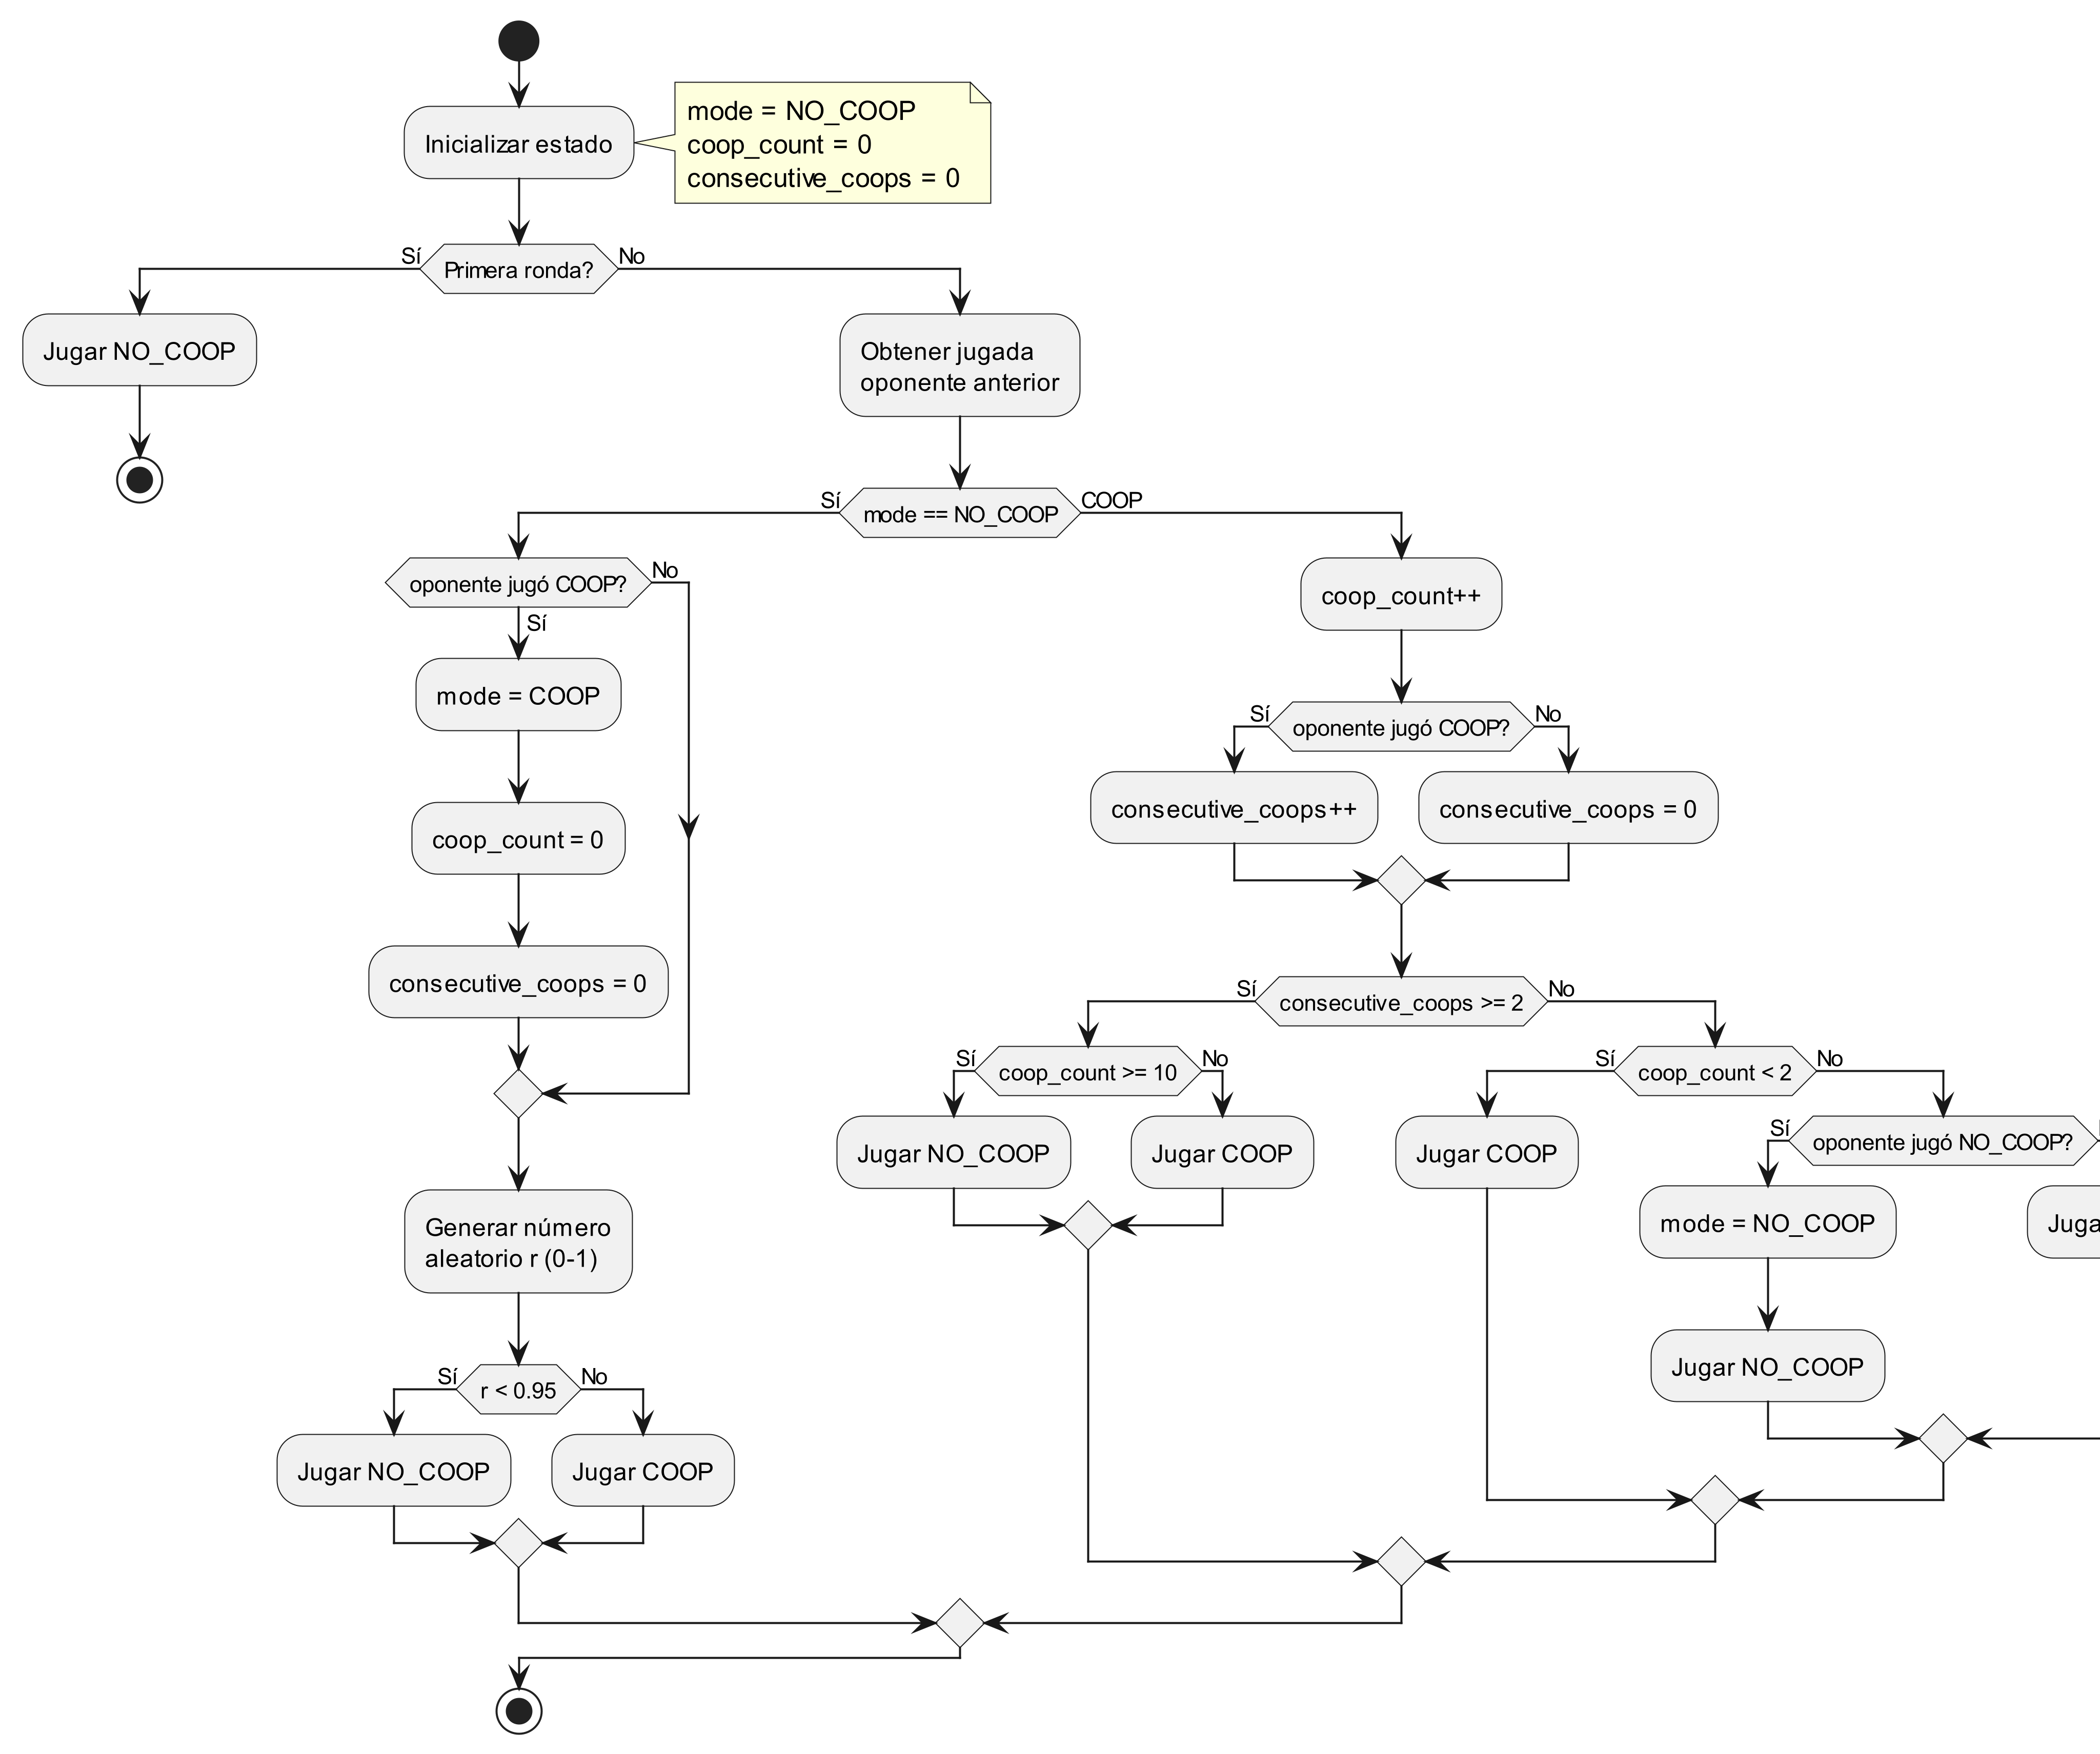
\includegraphics[width=0.96\textwidth]{diagrams/flow_convenceme.png}
  \caption{Diagrama de actividad del flujo del agente agente malévolo: Convenceme}
  \label{fig:flow_conven}
\end{figure}

\begin{figure}[H]        
  \centering             
  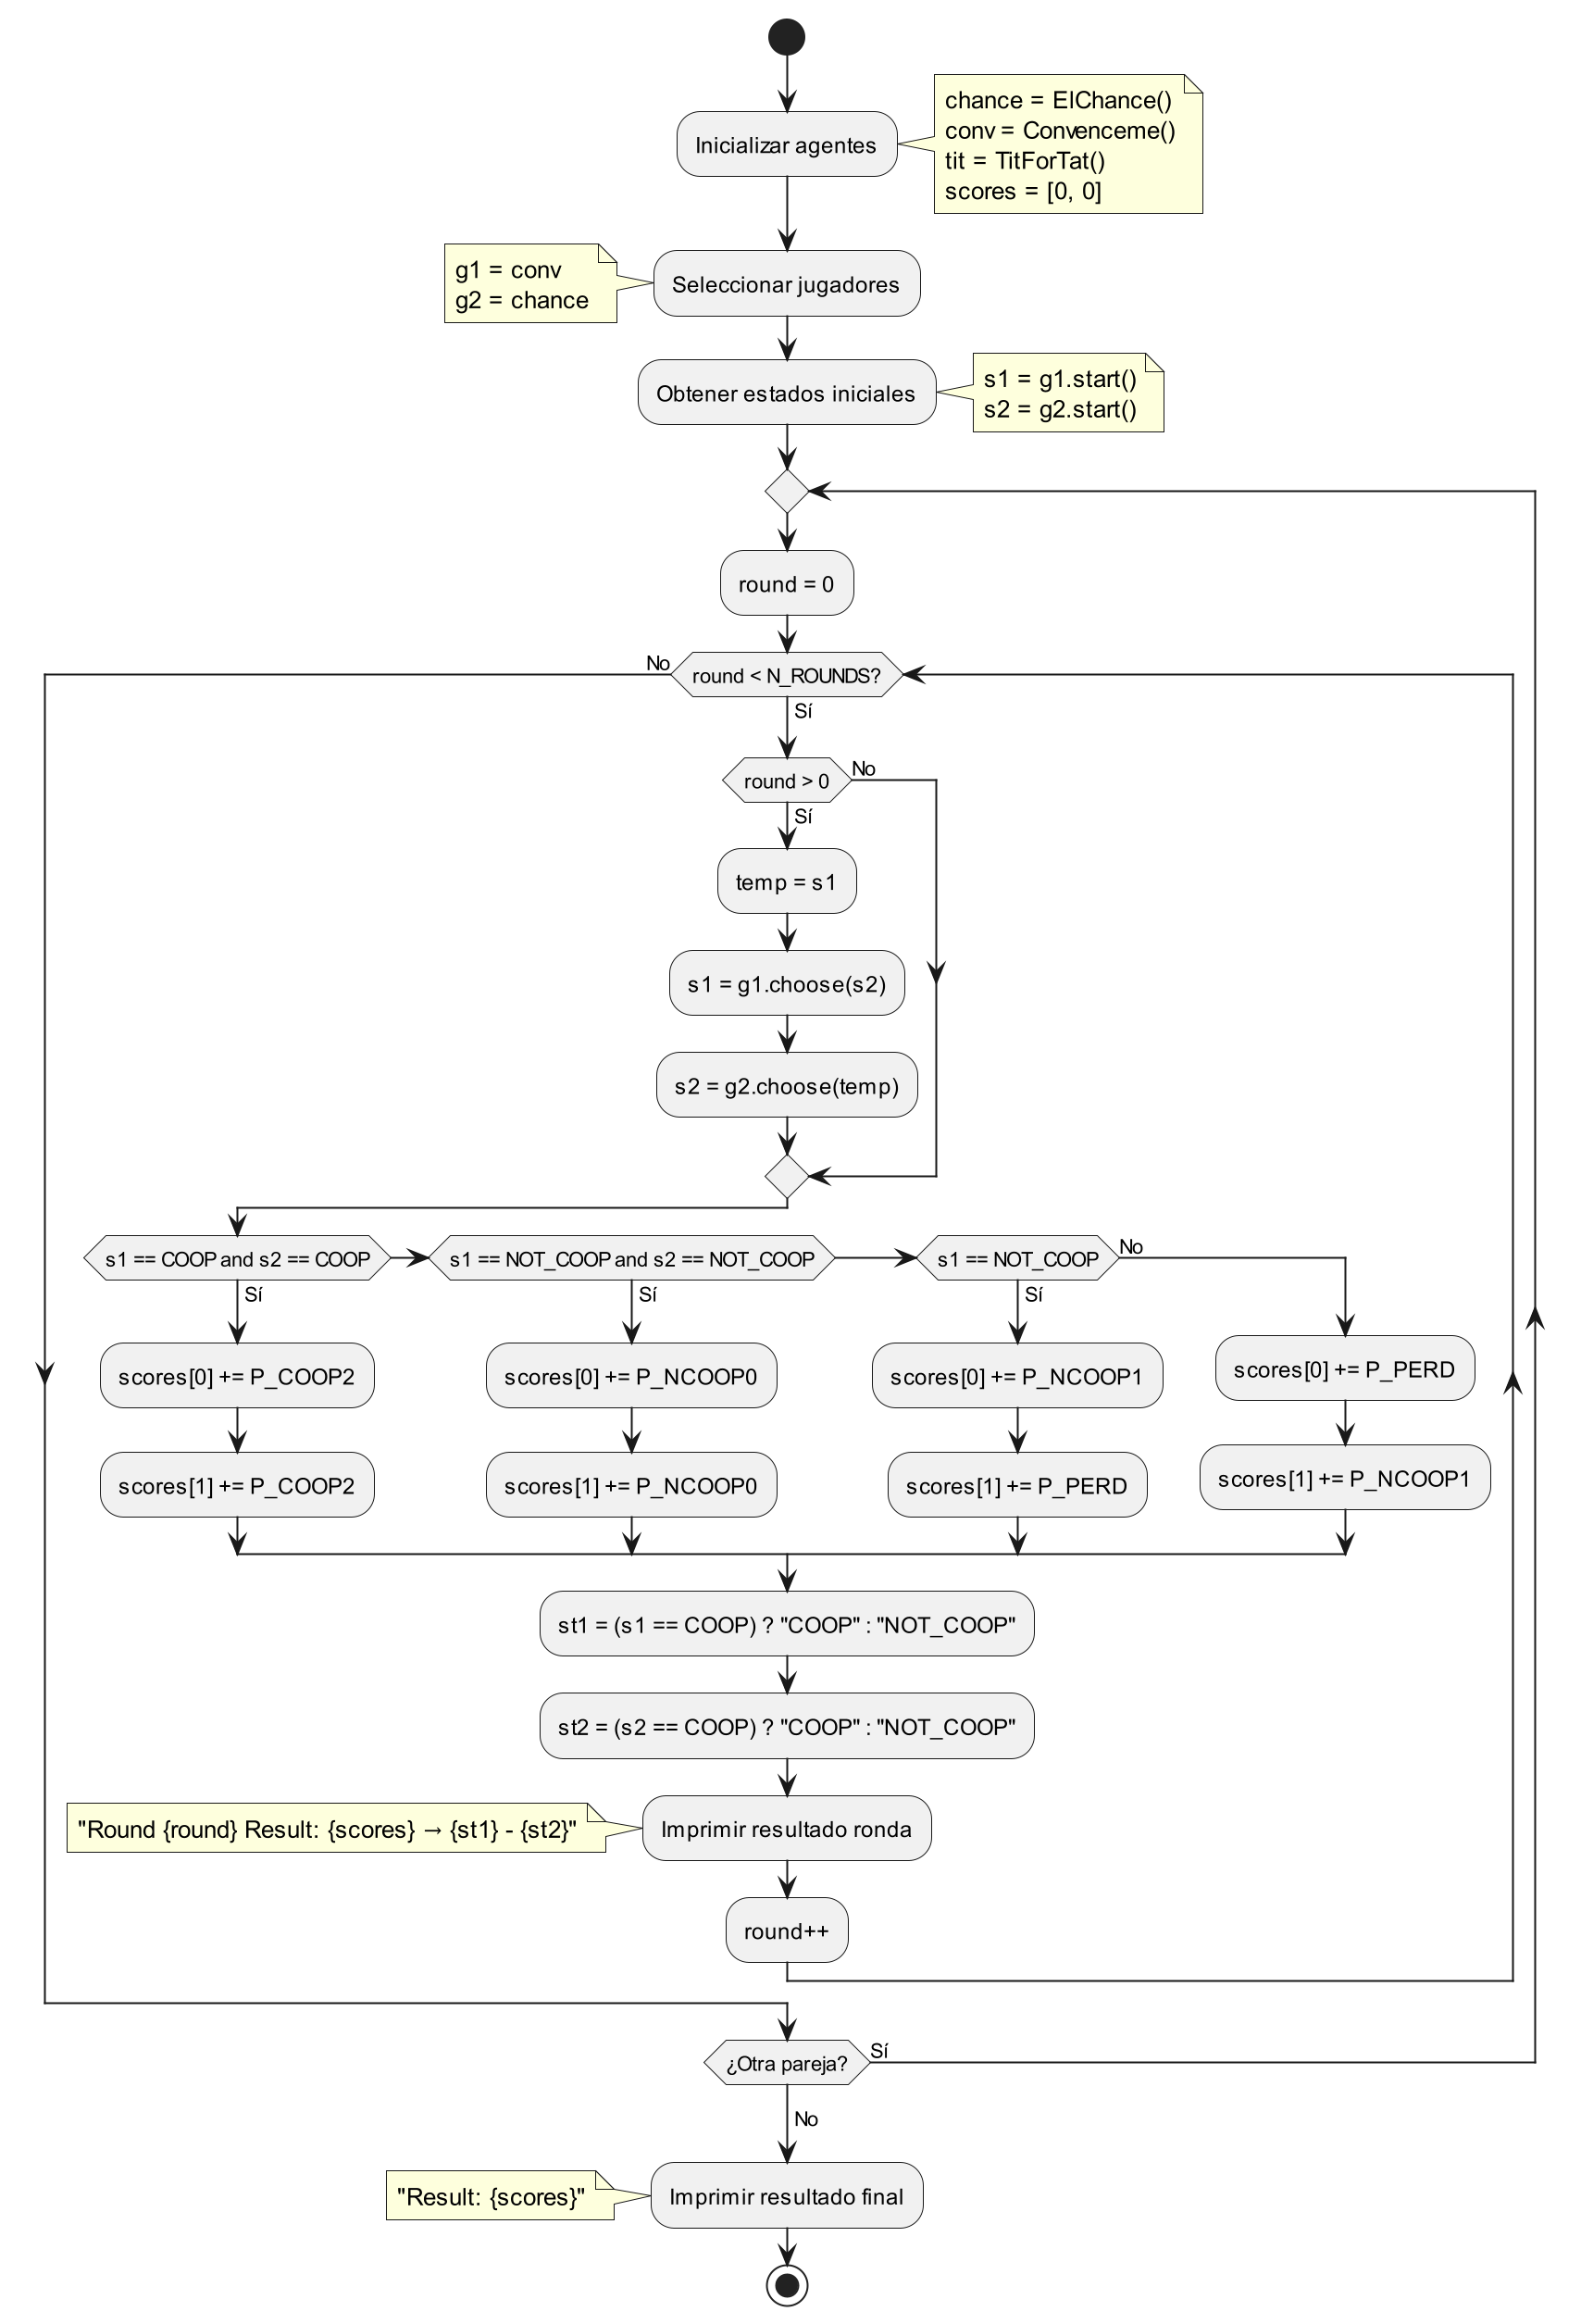
\includegraphics[width=0.8\textwidth]{diagrams/flow_tournament.png}
  \caption{Diagrama de actividad del flujo del torneo}
  \label{fig:flow_tourna}
\end{figure}

Este diseño modular facilita la incorporación de nuevas estrategias y 
la extensión de la simulación a variantes del Dilema del Prisionero.


%---------------------------------------------------------------------------------
% Código Fuente ---------------------------------------------------------
%---------------------------------------------------------------------------------

\section{Código Fuente}\label{sec:cod}

El código fuente completo de este modelo se encuentra adjunto en el buzón 
(31 Tarazona Jimenez Javier Andres 02.zip)
y disponible en el repositorio GitHub del proyecto:

\begin{center}
\url{https://github.com/JavierTarazona06/ME01_Tareas/tree/main/tarea31}
\end{center}

El repositorio incluye los siguientes componentes:

\begin{itemize}
  \item \texttt{agents.py}: implementación de las clases de agentes (\texttt{ElChance}, \texttt{Convenceme}, \texttt{TitForTat}) y sus métodos de decisión.
  \item \texttt{stochastics.py}: módulo para la generación de números aleatorios y distribución de Bernoulli.
  \item \texttt{main.py}: lógica principal del programa, que orquesta los torneos y registra los resultados.
  \item \texttt{graphics.py}: funciones para la generación de gráficos y visualización de puntuaciones.
  \item \texttt{requirements.txt}: lista de dependencias necesarias para instalar y ejecutar la aplicación.
  \item \texttt{tests/}: conjunto de escenarios de prueba y scripts de validación, junto con las gráficas resultantes de cada enfrentamiento.
\end{itemize}

%---------------------------------------------------------------------------------
% Manual Usuario ---------------------------------------------------------
%---------------------------------------------------------------------------------

\section{Manual Usuario}\label{sec:man_u}

El primer paso es descargar el archivo 
\texttt{31 Tarazona Jimenez Javier Andres 02.zip}.

Una vez descargado, descomprímalo y acceda a la carpeta. 
Dentro de ella, cree un 
entorno virtual utilizando Python 3.9. o superior. 
Para ello, ejecute el siguiente 
comando en 
la terminal o línea de comandos:

\begin{itemize}
  \item En Windows:
  \begin{verbatim}
    python3.12 -m venv nombre_del_entorno
  \end{verbatim}
  \item En macOS o Linux:
  \begin{verbatim}
    python3.12 -m venv nombre_del_entorno
  \end{verbatim}
\end{itemize}

Donde \texttt{nombre\_del\_entorno} es el nombre que desea asignar a 
su entorno virtual. 
A continuación, active el entorno virtual:

\begin{itemize}
  \item En Windows:
  \begin{verbatim}
    .\nombre_del_entorno\Scripts\activate
  \end{verbatim}
  \item En macOS o Linux:
  \begin{verbatim}
    source nombre_del_entorno/bin/activate
  \end{verbatim}
\end{itemize}


Una vez activo, instale  los requrimientos del proyecto
(numpy y matplolib) con el siguiente comando:

\begin{verbatim}
  pip install -r requirements.txt
\end{verbatim}


Ahora ya puede correr el programa ejecutando el archivo principal 
con el siguiente comando:

\begin{center}
  \begin{adjustbox}{minipage=\linewidth, center}
  \begin{verbatim}
    python main.py
  \end{verbatim}
  \end{adjustbox}
\end{center}

Al ejecutar va a pedir el path para guardar 
el resultado, 
preferiblemente indique un
archivo que termine en .txt.
Y luego va a
aparecer un menú en el cual puede seleccionar
que jugadores quiere poner a competir.

Los parámetros de números de rondas y puntajes,
se pueden cambiar desde main.py.

\begin{lstlisting}[language=Python]
N_ROUNDS = 200          # Número de rondas
P_COOP2 = 5             # Ganancia cuando los dos cooperan
P_NCOOP1 = 10           # Ganancia del ganador que traicionó (no cooperó)
P_PERD = 0              # Ganancia del que traicionaron (cooperó)
P_NCOOP0 = 2            # Ganancia cuando los dos no cooperan
\end{lstlisting}

Recuerde que los resultados se guardan en el path del archivo
indicado al iniciar el programa.

También se descarga una imagen \textit{"score\_players.png"} en la carpeta
de ejecución del programa donde se puede ver el histórico de
puntajes para los jugadores.

%---------------------------------------------------------------------------------
% Manual Técnico ---------------------------------------------------------
%---------------------------------------------------------------------------------

\section{Manual Técnico}\label{sec:man_t}


Este manual técnico describe los componentes internos del sistema 
de simulación del Dilema del Prisionero.

\subsection{Descripción de Módulos}
\begin{description}
  \item[\texttt{agents.py}] Contiene las clases base y derivadas de agentes:
    \texttt{Agente}, \texttt{ElChance}, \texttt{Convenceme}, \texttt{TitForTat}. Cada clase implementa los métodos \texttt{start()} y \texttt{choose()} según su estrategia.
  \item[\texttt{stochastics.py}] Proporciona funciones de generación de números aleatorios:
    distribución de Bernoulli y generador de punto flotante uniforme en [0,1) sin usar \texttt{random}.
  \item[\texttt{main.py}] Orquesta la simulación:
    \begin{itemize}
      \item Define el menú de selección de agentes.
      \item Ejecuta la función \texttt{torneo(agentes, n\_rondas)}.
      \item Registra y guarda resultados en archivos \texttt{.txt} y \texttt{.png} dentro de \texttt{tests/}.
            Aunque realmente es en los archivos especificados.
    \end{itemize}
  \item[\texttt{graphics.py}] Incluye utilidades para:
    \begin{itemize}
      \item Cargar resultados de \texttt{.csv}.
      \item Generar gráficos de líneas de puntajes acumulados.
    \end{itemize}
  \item[\texttt{tests/}] Carpeta que contiene:
    \begin{itemize}
      \item Archivos de resultados de escenarios (	exttt{escenario1.txt}, etc.).
      \item Gráficas generadas para cada escenario.
    \end{itemize}
\end{description}

%---------------------------------------------------------------------------------
% Experimentación ---------------------------------------------------------
%---------------------------------------------------------------------------------

\section{Experimentación}\label{sec:exp}

La experimentación consistió en enfrentamientos de 200 rondas entre las 
dos estrategias propuestas la benévola \texttt{ElChance} y la malévola 
\texttt{Convenceme} y, de manera adicional, enfrentamientos de cada una 
contra \texttt{TitForTat}. En cada torneo se recogieron el historial 
de puntajes por ronda, el puntaje total acumulado, la tasa de 
cooperación y las victorias relativas, con el fin de determinar 
cuál estrategia resultaba más eficiente, entendida como la que acumula 
más puntos. Además, se verificó que cada estrategia cumpliera los 
criterios de una buena estrategia eficiente:  
\begin{itemize}  
  \item Iniciar cooperando y tender hacia la cooperación.  
  \item Ser indulgente: no cooperar tras una traición, 
        pero sin rencor prolongado.  
  \item Ser vengativa: castigar con no cooperación cuando el 
        oponente traiciona.  
  \item Mantener un algoritmo claro y bien definido.  
\end{itemize}  
Cada torneo se repitió cinco veces, obteniéndose resultados 
consistentes en todas las ejecuciones.

\subsection{Análisis de resultados}

\subsubsection{Escenario 1: Confrontación 
  \texttt{1. ElChance} vs. \texttt{2. Convenceme}}\label{sec:esc1}

El historial de puntajes se muestra en la Figura~\ref{fig:scores_essc1}. 
Tras 200 rondas, \texttt{ElChance} acumuló 935 puntos, 
mientras que \texttt{Convenceme} alcanzó 1065 puntos, 
imponiéndose claramente en el enfrentamiento.  

Las tasas de cooperación resultaron ser del 96\% para 
\texttt{ElChance} y del 90\% para \texttt{Convenceme}. 
En cuanto a las victorias relativas, veces en que cada agente obtuvo 
mayor puntaje al traicionar al oponente, se registraron 7 para 
\texttt{ElChance} y 19 para \texttt{Convenceme}.  

Estos resultados indican que, aunque \texttt{ElChance} mostró un 
fuerte sesgo hacia la cooperación (cumpliendo el criterio de iniciar 
cooperando y tender a cooperar por ser benévola), su excesiva indulgencia 
frente a las traiciones de \texttt{Convenceme} le restó eficacia. 
Por el contrario, \texttt{Convenceme}, al aplicar un castigo 
más contundente (mayor número de victorias relativas) y mantener 
un comportamiento claro y agresivo, resultó ser más eficiente en 
términos de puntuación acumulada.

\begin{figure}[H]        
  \centering             
  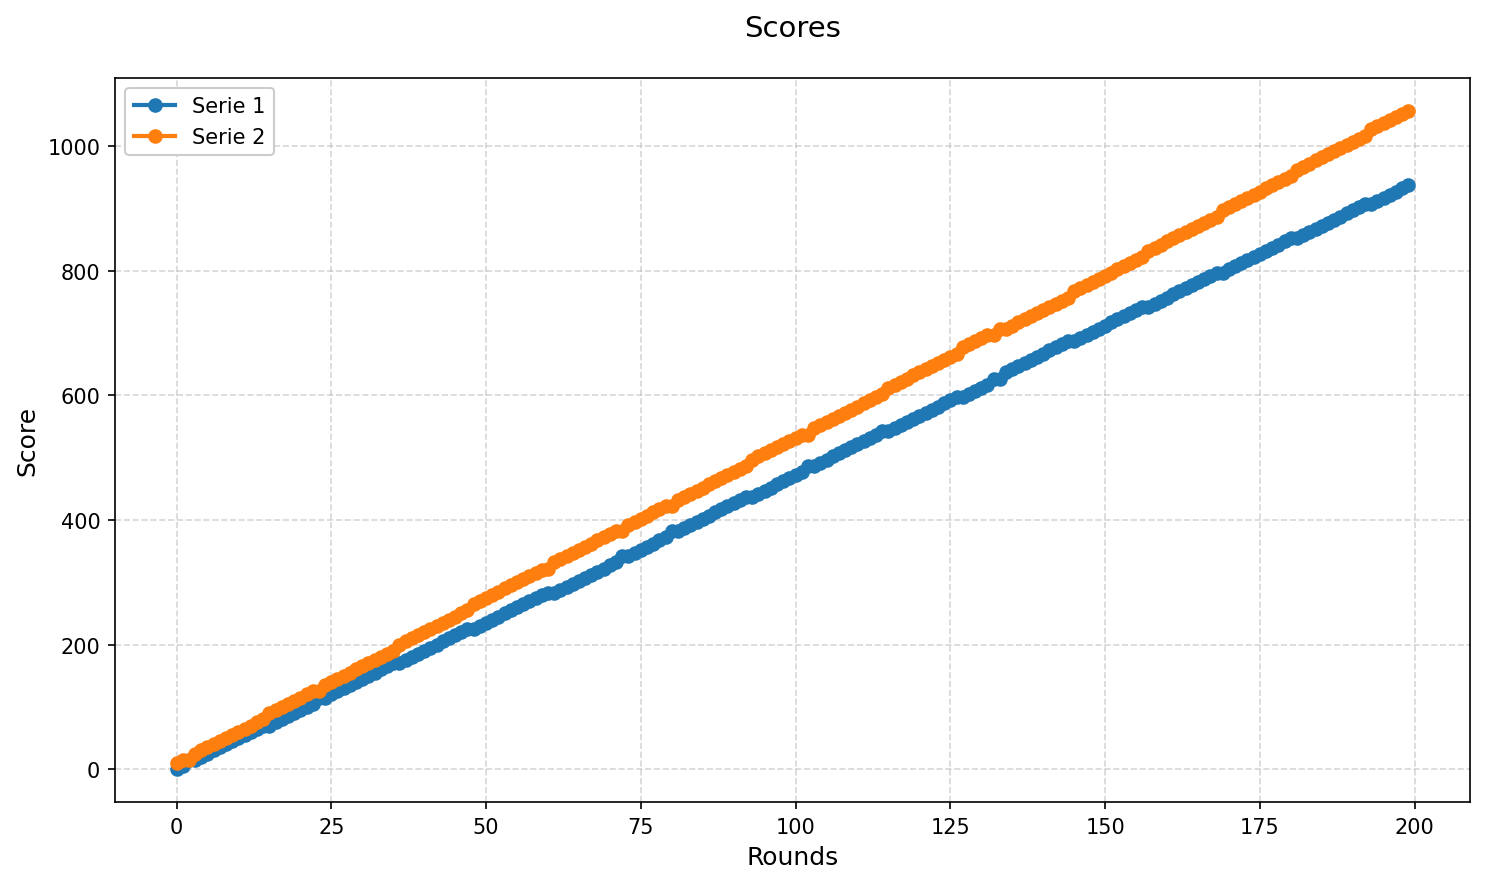
\includegraphics[width=0.8\textwidth]{diagrams/escenario1.png}
  \caption{Puntajes acumulados del escenario de prueba 1}
  \label{fig:scores_essc1}
\end{figure}

\subsubsection{Escenario 2: Confrontación 
  \texttt{1. ElChance} vs. \texttt{2. Tit for Tat}} \label{sec:esc2}

En este caso se busca comparar la estrategia benévola con la mencionada 
\texttt{TitForTat} como la más eficiente. El historial de puntajes se muestra en 
la Figura~\ref{fig:scores_essc2}. Tras 200 rondas, \texttt{ElChance} acumuló 1000 puntos, 
mientras que \texttt{TitForTat} alcanzó también 1000 puntos, resultando en un empate claro.

Las tasas de cooperación fueron del 98\% para ambos. En cuanto a las victorias relativas, 
veces en que cada agente obtuvo mayor puntaje al traicionar al oponente, se registraron 4 para 
cada uno.

Estos resultados indican que, aunque el comportamiento de \texttt{ElChance} coincide 
con lo descrito en el escenario~\ref{sec:esc1}, \texttt{TitForTat} actúa con 
una estrategia óptima, tal como se esperaba: es una estrategia sólida, indulgente, 
clara y vengativa sin rencor. No perdona ninguna traición, pero coopera cuando es 
necesario, lo cual le permitió, al menos, empatar.

\begin{figure}[H]        
  \centering             
  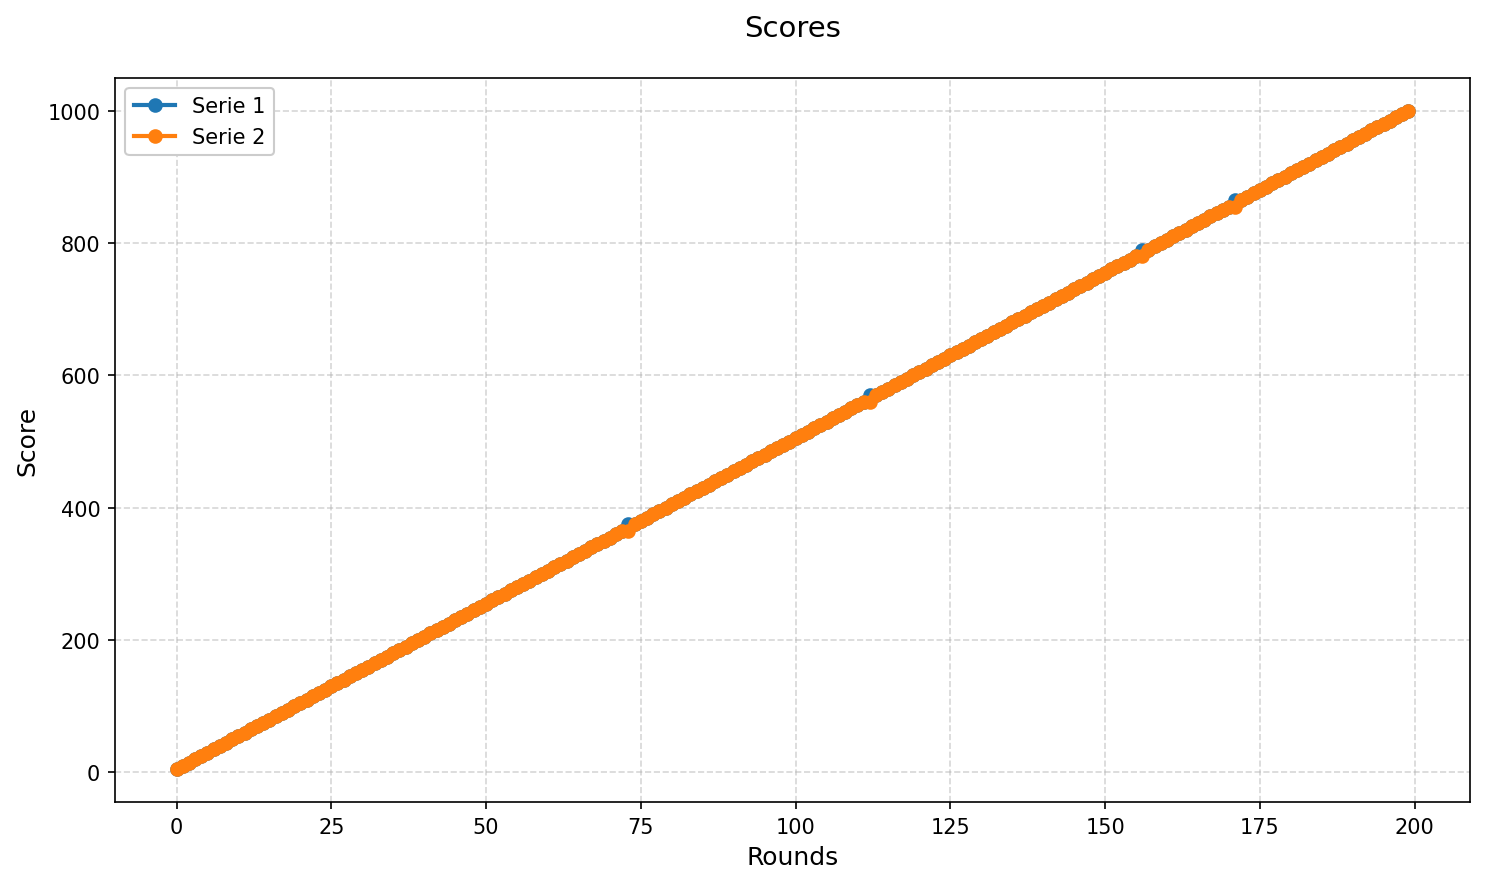
\includegraphics[width=0.8\textwidth]{diagrams/escenario2.png}
  \caption{Puntajes acumulados del escenario de prueba 2}
  \label{fig:scores_essc2}
\end{figure}
 
\subsubsection{Escenario 3: Confrontación 
  \texttt{1. Convenceme} vs. \texttt{2.Tit for Tat}}\label{sec:esc3}

En este escenario, considerado el más relevante, se compara la estrategia malévola 
\texttt{Convenceme}, ganadora del escenario~\ref{sec:esc1}, contra \texttt{TitForTat}, 
en torneos de 200 rondas. El historial de puntajes aparece en la 
Figura~\ref{fig:scores_essc3}. Tras 200 rondas, ambos agentes acumularon 1000 puntos, 
resultando en un empate.

Las tasas de cooperación fueron idénticas, del 95,5\% para cada uno. 
Esto se explica porque \texttt{Convenceme} coopera con menor frecuencia 
que \texttt{ElChance} (ver sección~\ref{sec:esc2}), mientras que 
\texttt{TitForTat} replica fielmente la acción del oponente. 
En cuanto a las victorias relativas, ocasiones en que cada agente obtuvo 
un mayor puntaje no cooperando, se registraron 9 para ambos competidores.

Estos resultados indican que la no cooperación espontánea 
incrementa las victorias individuales, lo que explica la victoria de 
\texttt{Convenceme} sobre \texttt{ElChance} en el escenario~\ref{sec:esc1}, 
pero su empate frente a \texttt{TitForTat} en este tercer escenario. 
Asimismo, se confirma que \texttt{TitForTat} mantiene su eficiencia: 
inicia cooperando, castiga a la traición sin rencor prolongado y 
coopera cuando corresponde, lo que le permitió empatar 
también con \texttt{Convenceme}.

\begin{figure}[H]        
  \centering             
  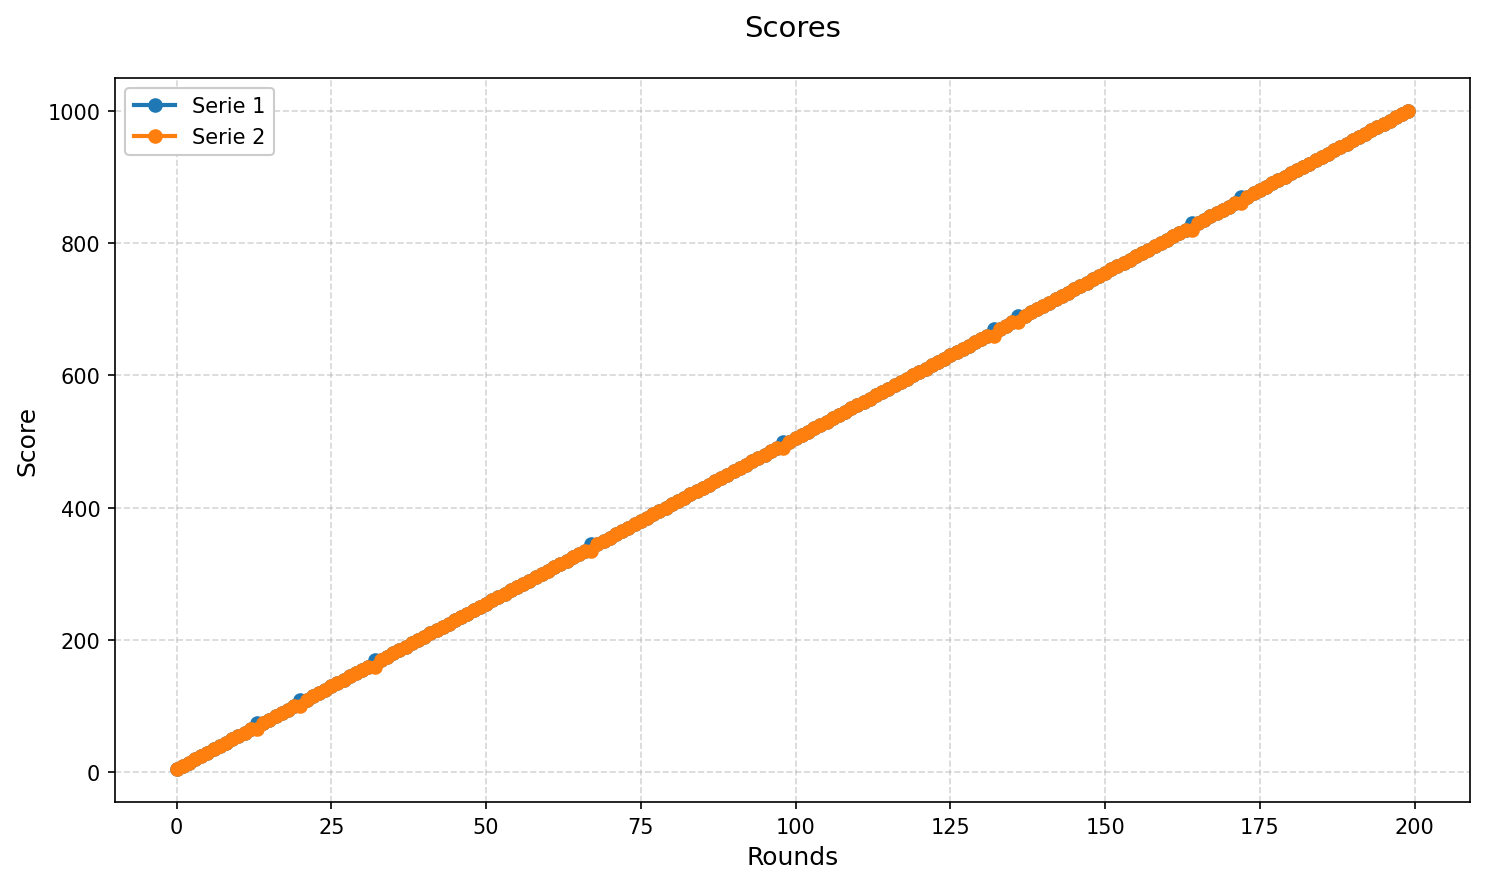
\includegraphics[width=0.8\textwidth]{diagrams/escenario3.png}
  \caption{Puntajes acumulados del escenario de prueba 3}
  \label{fig:scores_essc3}
\end{figure}

\subsection{Análisis de los resultados}

En el conjunto de los tres escenarios evaluados, cada estrategia mostró fortalezas y 
debilidades que permiten establecer conclusiones precisas sobre su eficiencia relativa. 
En el Escenario~\ref{sec:esc1}, \texttt{Convenceme} se impuso frente a \texttt{ElChance} 
gracias a su agresividad controlada y a un mayor número de victorias relativas 
(19 contra 7), acumulando 1065 puntos frente a 935 de la estrategia benévola. 
No obstante, al competir contra \texttt{TitForTat} (Escenarios~\ref{sec:esc2} y \ref{sec:esc3}), 
\texttt{Convenceme} empata con 1000 puntos, 
lo que evidencia un límite en su ventaja cuando se enfrenta a un oponente que 
replica con fidelidad cada traición o cooperación.

Desde la perspectiva de las métricas de cooperación y estabilidad,
\texttt{ElChance} alcanzó la tasa más alta de colaboración 
(96–98 \%), pero su excesiva indulgencia (“perdona” traiciones con demasiada frecuencia) 
le penalizó frente a agentes más punitivos. Por su parte, \texttt{Convenceme} 
mantiene una tasa de cooperación moderada (90–95,5 \%), balance que le permitió maximizar 
victorias individuales sin descuidar por completo la reciprocidad. Sin embargo, el comportamiento 
de \texttt{TitForTat}, cooperar inicialmente, castigar con una única respuesta negativa y 
luego volver a cooperar, demostró ser el más sólido: su tasa de cooperación
 constante (95,5–98 \%) y su capacidad de no ceder ventaja (nunca pierde, siempre empata o gana) 
 lo convierten en la estrategia más eficiente según los criterios establecidos.

En términos de eficiencia global, definir una buena estrategia implica no solo maximizar 
el puntaje, sino también garantizar un comportamiento predecible y resistente a 
distintos estilos de juego. \texttt{TitForTat} cumple con estos requisitos:  
\begin{itemize}  
  \item Inicia cooperando y favorece la cooperación mutua.  
  \item Responde a la traición con un castigo inmediato, sin prolongar el rencor.  
  \item Mantiene un algoritmo simple y transparente, fácil de implementar y extender.  
\end{itemize}  
Por ello, a pesar de que \texttt{Convenceme} logró el mayor puntaje en el torneo 
global (al enfrentarse a tres oponentes distintos), \texttt{TitForTat} se mantiene como
la estrategia más eficiente de forma consistente: si no gana, al menos empata, asegurando 
un rendimiento estable en cualquier emparejamiento.

Finalmente, estos resultados sugieren que, en entornos donde coexisten múltiples estilos 
de juego, las estrategias basadas en reciprocidad estricta ofrecen un equilibrio óptimo 
entre generosidad y represalia.

\section{Conclusión}\label{sec:conclusion}

En este trabajo se implementaron y compararon tres estrategias para el 
Dilema del Prisionero: \texttt{ElChance}, \texttt{Convenceme} y \texttt{TitForTat}
 mediante simulaciones iteradas de 200 rondas y torneos repetidos cinco veces. 
 Los análisis de historial de puntajes, tasas de cooperación y victorias
  relativas mostraron lo siguiente:

\begin{itemize}
  \item \texttt{ElChance} destacó por su alta generosidad, con tasas de 
  cooperación entre el 96\,\% y el 98\,\%, pero su excesiva indulgencia le 
  restó puntos frente al oponente más agresivo.
  \item \texttt{Convenceme} obtuvo el mayor puntaje global (1057) debido a su carácter 
  agresivo y al diseño de emparejamientos, equilibrando una cooperación moderada 
  (90\,--\,95,5\,\%) con un alto número de victorias relativas.
  \item \texttt{TitForTat} mantuvo una eficiencia constante: tasas de cooperación
   del 95,5\,\% al 98\,\%, y nunca perdió un enfrentamiento (empató en todos los escenarios).  
\end{itemize}

Si bien \texttt{Convenceme} acumuló más puntos en el torneo global, 
\texttt{TitForTat} se confirma como la estrategia más eficiente según
 los criterios de robustez y predictibilidad: si no gana, al menos empata. 
 Su simplicidad algorítmica, iniciar cooperando, responder a la traición con un 
 único castigo y volver a cooperar, la convierte en la opción óptima para 
 entornos en los que coexisten distintos estilos de juego.

\medskip

Sería interesante explorar variantes de 
\texttt{TitForTat} con memoria de longitud variable, introducir ruido en las decisiones, 
ampliar el número de jugadores o incorporar mecanismos de reputación más complejos, 
con el fin de evaluar la resistencia y adaptabilidad de las estrategias en contextos 
aún más variados.  


\section{Referencias}
\renewcommand{\refname}{}

\begin{thebibliography}{9}

\bibitem{ref} \label{ref:vidIntro} Veritasium en español, “Lo que el Dilema del Prisionero Revela 
Sobre la Vida, el Universo y Todo lo Demás,” YouTube video, 7:03, Mar. 2024. [Online]. 
Available: \url{https://youtu.be/vBgrvVY1jGo}

\bibitem{ref} \label{ref:just} R. Axelrod, The Evolution of Cooperation. New York: 
Basic Books, 1984.

\end{thebibliography}

\end{document}